% TODO: Say we can load pgm maps from ROS 2

\section{Simple Simulator}
The simple simulator was developed as an easy way to test and debug the behavior of a robot swarm given a robot behavior. It is runs a simple 2D simulation with a time step for 60 times pr. simulated second in a multi threaded manner. Robots are represented as circles, with their id marked in the middle. \Cref{fig:simple-sim-interface} shows the user interface if the simple simulator.

\begin{figure}
    \begin{center}
        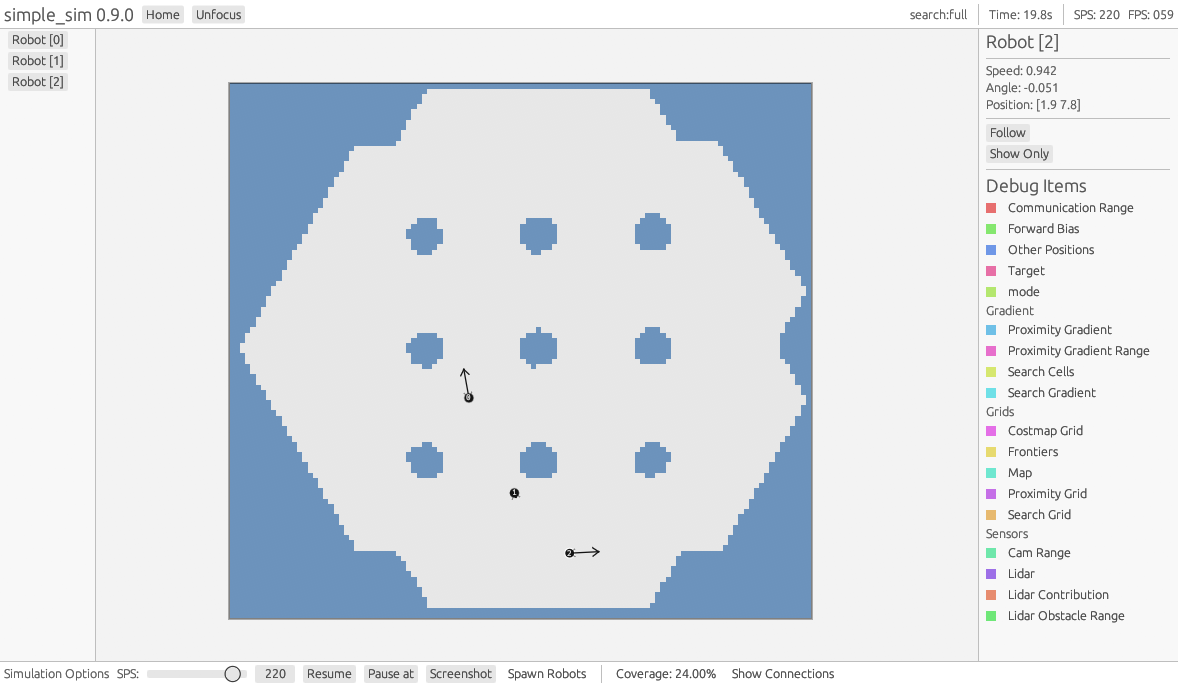
\includegraphics[width=0.95\textwidth]{figures/simple-sim-gui.png}
    \end{center}
    \caption{Simple simulator interface as it simulates three robots in the left part of the map.}\label{fig:simple-sim-interface}
\end{figure}


\subsection{Sensor Approximation}
Running a robot's behavior requires pose, LiDAR and camera inputs. Pose is set directly by the simulator and does therfore not require much implementation. LiDAR and camera are both implemented using ray marching {\color{red} [CITE??]}. Lidar is approximated by casting rays around the robot with a fixed angle step and marching along each until the ray hits an object as seen on \cref{fig:lidar-approximation}.

% TODO: Write about camera approximation

\begin{figure}
    \centering

    \begin{subfigure}[b]{0.45\textwidth}
        \centering
        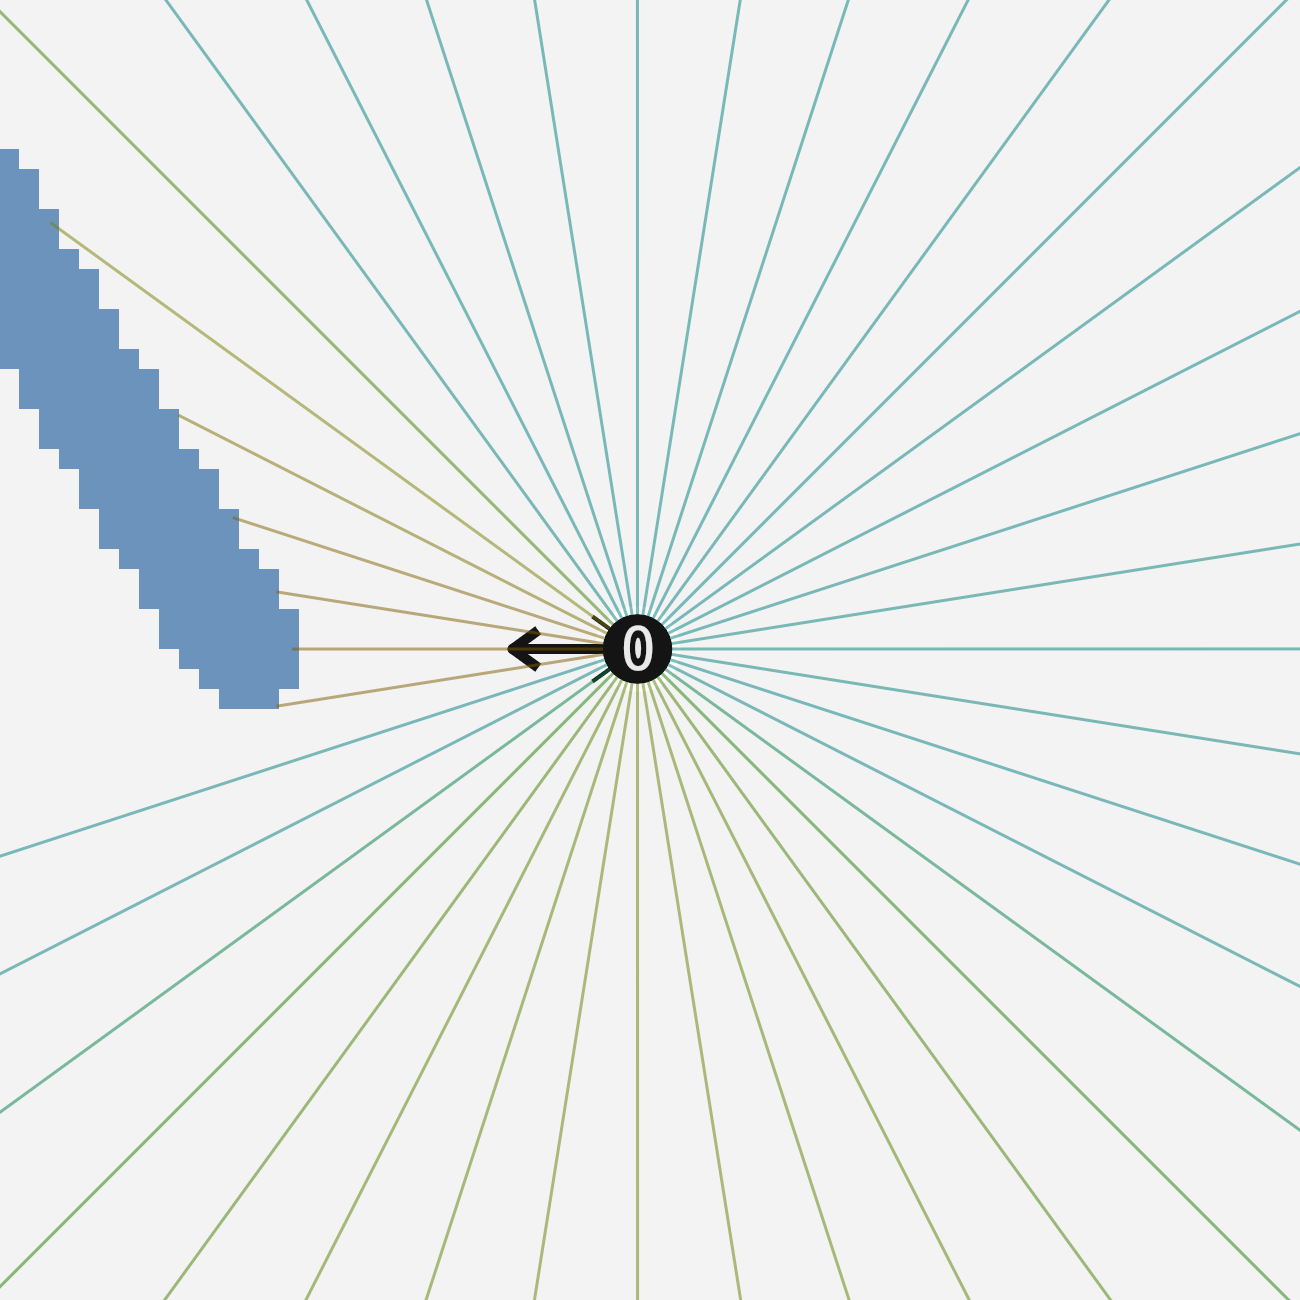
\includegraphics[width=\textwidth]{figures/simple-lidar.png}
        \caption{LiDAR approximation}
        \label{fig:lidar-approximation}
    \end{subfigure}
    \begin{subfigure}[b]{0.45\textwidth}
        \centering
        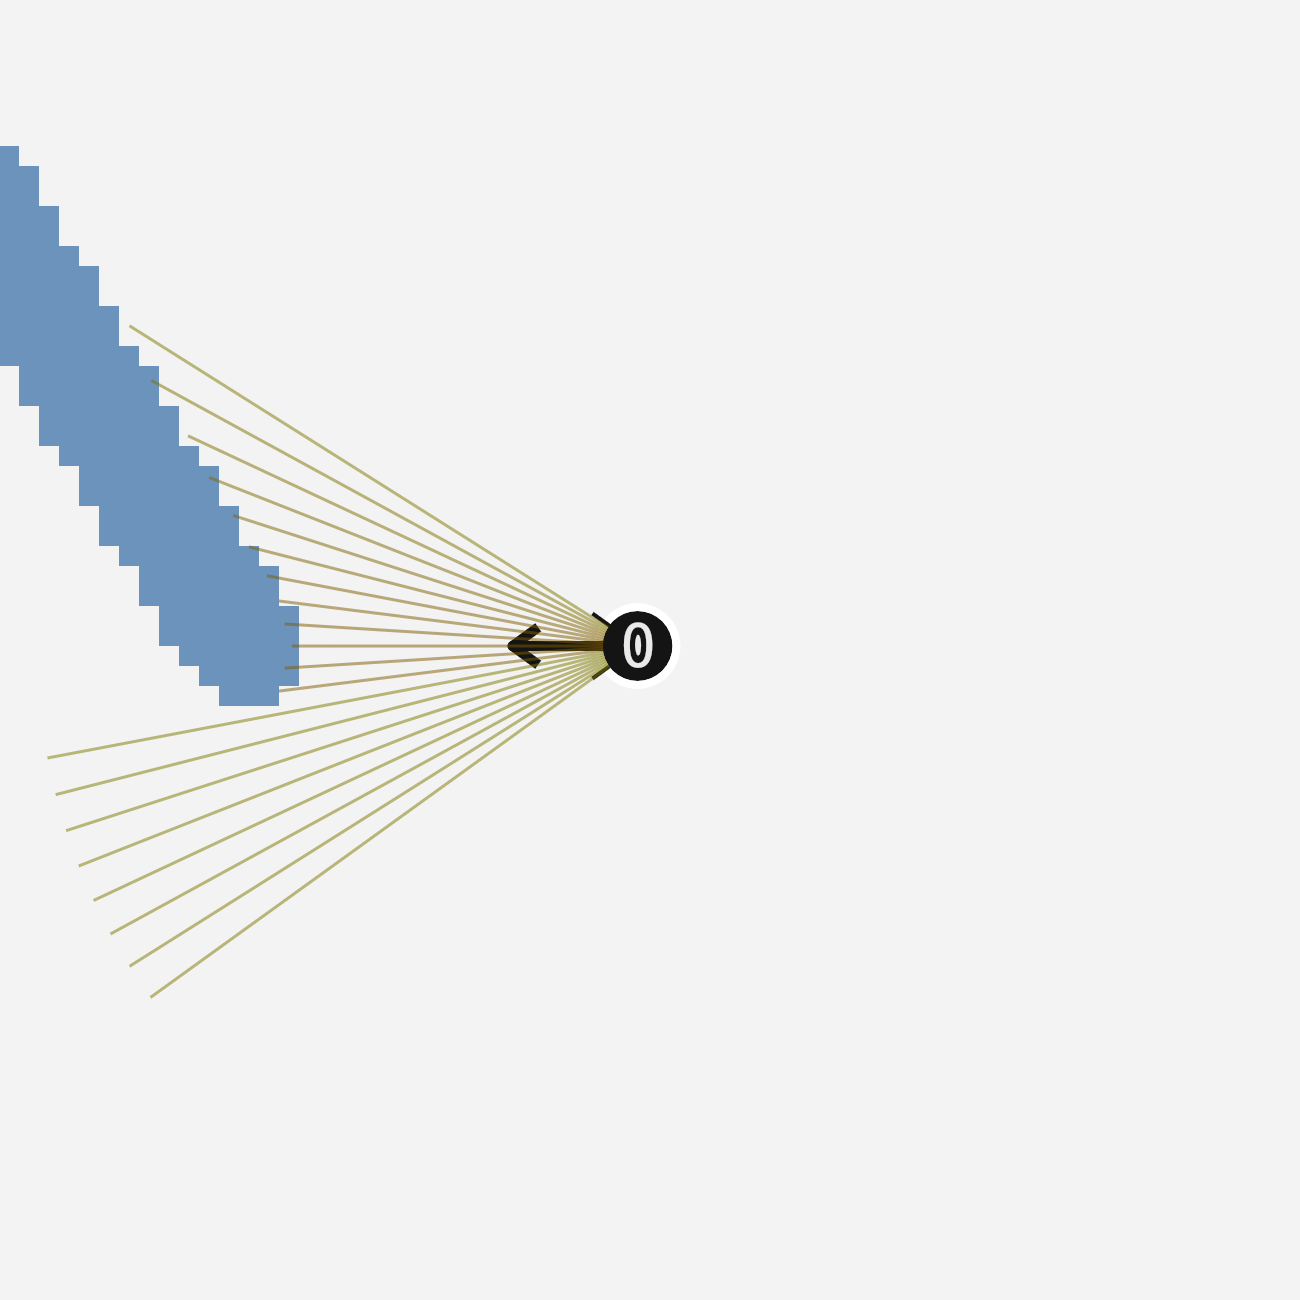
\includegraphics[width=\textwidth]{figures/simple-camera.png}
        \caption{Camera approximation}
        \label{fig:camera-approximation}
    \end{subfigure}

    \caption{LiDAR and camera simulated in the simple simulator.}\label{fig:sensor-approximation}
\end{figure}



% Debugging
% Library
